\documentclass[specialist,
               substylefile = spbu.rtx,
               subf,href,colorlinks=true, 12pt]{disser}

\usepackage[a4paper,
            mag=1000, includefoot,
            left=3cm, right=1.5cm, top=2cm, bottom=2cm, headsep=1cm, footskip=1cm]{geometry}
\usepackage[T2A]{fontenc}
\usepackage[utf8]{inputenc}
\usepackage[english,russian]{babel}
\ifpdf\usepackage{epstopdf}\fi

% Использовать полужирное начертание для векторов
\let\vec=\mathbf

% Включать подсекции в оглавление
\setcounter{tocdepth}{2}

\usepackage[defaultmono]{droidmono}
\usepackage[T2A]{fontenc}
% \usepackage{csquotes}

\usepackage[intlimits]{amsmath}
\usepackage{amsfonts}
\usepackage{amssymb}
\usepackage{amsthm}

\usepackage{algorithm2e}
\usepackage{graphicx}
\graphicspath{ {media/} }
\usepackage{color}

\usepackage[fixlanguage]{babelbib}
\selectbiblanguage{russian}

% \usepackage{natbib}
% \usepackage[style=numeric]{biblatex}
% \addbibresource{biblio-u.bib}

\usepackage{hyperref}
\newtheorem{theorem}{Теорема}
\newcommand{\ev}{\mathsf{E}}
\newcommand{\R}{\ensuremath{\mathbb{R}}}

% \renewcommand\topfraction{0.85}
% \renewcommand\bottomfraction{0.85}
% \renewcommand\textfraction{0.1}
% \renewcommand\floatpagefraction{0.85}
\setlength\parindent{0pt}
\setlength\parskip{0.5em}

% \usepackage{minted}
\usepackage{listings}
\lstdefinestyle{customjava}{
%   belowcaptionskip=1\baselineskip,
  	breaklines=true,
  	breakatwhitespace=true,
%   xleftmargin=\parindent,
%   language=Java,
%   showstringspaces=false,
   	basicstyle=\footnotesize\fdmfamily,
   	keywordstyle=\bfseries\color{blue},
  	commentstyle=\color{magenta},
  	morekeywords={ImitatedAsset, },
  	% identifierstyle=\color{green},
%   stringstyle=\color{orange},
}
\lstset{style=customjava, language=Java}

\usepackage{tikz}
\usetikzlibrary{arrows}
\usetikzlibrary{positioning}

%----------------------------------------------------------------
\begin{document}

%
% Титульный лист на русском языке
%

% Название организации
\institution{%
    Правительство Российской Федерации \\
    Федеральное государственное бюджетное образовательное учреждение \\
    высшего профессионального образования \\
    «Санкт-Петербургский государственный университет» \\
    Кафедра статистического моделирования
}

\title{Отчет о научно-исследовательской практике}

% Тема
\topic{\normalfont\scshape%
    Имитационная модель американского опциона}

% Автор
\author{Миллер Анастасия Александровна}

% Научный руководитель
\sa       {С.\,М.~Ермаков}
\sastatus {д.\,ф.-м.\,н., профессор}

% Город и год
\city{Санкт-Петербург}
\date{\number\year}

\maketitle

\tableofcontents

\intro
    \par Задачами семестра являлись реализация и сравнение методов оценки цены американского опциона. В главе 1 содержится краткое описание исходного метода и оценок, численные результаты реализации, в главе 2 --- описание модифицированных методов и оценок, численные результаты их реализации. Глава 2 является описанием результатов работы в течение семестра.
\chapter{Метод случайных деревьев}
	\section{Обозначения и умолчания}
	\par Будем строить модель на примере американского опциона с конечным числом дат погашения $t_1, \ldots t_m$ (также называемого бермудским опционом). Мы также сузим класс решаемых нами задач до тех, в которых вся необходимая информация об активе, на который выписан рассматриваемый опцион, может быть представлена в виде Марковского процесса $S\left( t \right), t \in \left\lbrace t_i \right\rbrace_{i = 1}^m$ со значениями в $\mathbb{R}^d$. Для уменьшения объёма текста будем обозначать $S\left(t_i\right) \equiv S_i$. Положим также $h_i\left(x\right)$ --- дисконтированный размер выплаты по опциону в момент $t_i$ при том, что $x = S_i$ и опцион не был исполнен до этого, $V_i\left(x\right)$ --- стоимость опциона в момент $t_i$ при том, что $x = S_i$.
	\par Нетрудно видеть, что
		\begin{eqnarray}\label{eq:option-recursive}
			V_m\left(x\right) = h_m\left(x\right), \\
			V_{i-1}\left(x\right) = \max\left\lbrace h_{i-1}\left(x\right), \mathsf{E}\left[V_i\left(S_i\right)|S_{i-1}=x\right]\right\rbrace
		\end{eqnarray}
	 --- на каждом шаге мы выбираем наиболее выгодное решение. $V_0\left(S_0\right)$ --- цена опциона с $m$ датами исполнения.
	\paragraph{Оценки} В \cite{Broadie1997} предложены оценки сверху и снизу $\hat{V}_0$ и $\hat{v}_0$ и доказана их состоятельность и асимптотическая несмещённость для $V_0\left(S_0\right)$.
	\begin{align}\label{eq:upper}
		\hat{V}_m^{j_1 \ldots j_m} &= h_m\left(S_m^{j_1 \ldots j_m}\right), \\
		\hat{V}_i^{j_1 \ldots j_i} &= \max \left\lbrace h_i \left( S_i^{j_1 \ldots j_i} \right), \frac{1}{b} \sum_{j = 1}^b \hat{V}_{i+1}^{j_1 \ldots j_i j}\right\rbrace,
	\end{align}
	\begin{align}\label{eq:lower}
		\hat{v}_m^{j_1 j_2 \cdots j_m} &= h\left( S_m^{j_1 j_2 \cdots j_m}\right), \\
		\hat{v}_{ik}^{j_1 j_2 \cdots j_i} &= \left\lbrace
				    \begin{array}{l l}
					    h\left( S_i^{j_1 j_2 \cdots j_i}\right), & \, \text{если } \frac{1}{b-1}\sum_{j=1, j\not= k}^b \hat{v}_{i+1}^{j_1 j_2 \cdots j_i j} \leq h\left(S_i^{j_1 j_2 \cdots j_i}\right), \\
					    \hat{v}_{i+1}^{j_1 j_2 \cdots j_i k}, & \, \text{иначе}
				    \end{array}\right. \\
		\hat{v}_i^{j_1 j_2 \cdots j_i} &= \frac{1}{b}\sum_{k=1}^b \hat{v}_{ik}^{j_1 j_2 \cdots j_i}.
	\end{align}

	\section{Построение дерева}
	\par Метод случайного дерева основан на моделировании цепи $S_0, S_1, \ldots S_n$ состояний актива. Зафиксируем параметр ветвления $b$. Из исходного состояния $S_0$ смоделируем $b$ независимых следующих состояний $S_1^1, S_1^2, \ldots S_1^b$, все с условием $S_0$. Для каждого $S_1^i$ снова смоделируем $b$ независимых последующих состояний $S_2^{i1}, \ldots S_2^{ib}$. На $m$-ом шаге будем иметь $b^m$ состояний, и это и есть источник основного недостатка этого метода --- его экспоненциальной алгоритмической сложности. Пример дерева можно увидеть на рис. \ref{fig:exponentialTree}.
	\begin{figure}[h]
	    \centering
		\includegraphics[width=0.8\textwidth, height=0.15\paperheight]{tree_sample.pdf}
		\caption{Выбор вершин по квантилям эмпирического распределения}
		\label{fig:exponentialTree}
	\end{figure}
	\par Таким образом, мы имеем дерево с $\sum_{k=1}^m b^k = \frac{b\left(b^m-1\right)}{b-1} = O\left(b^m\right)$ вершинами и две оценки искомой величины по этому дереву. Классический алгоритм реализован, результаты его работы представлены на рис. \ref{fig:true_value_test_standard}.
	\begin{figure}[h]
	    \centering
		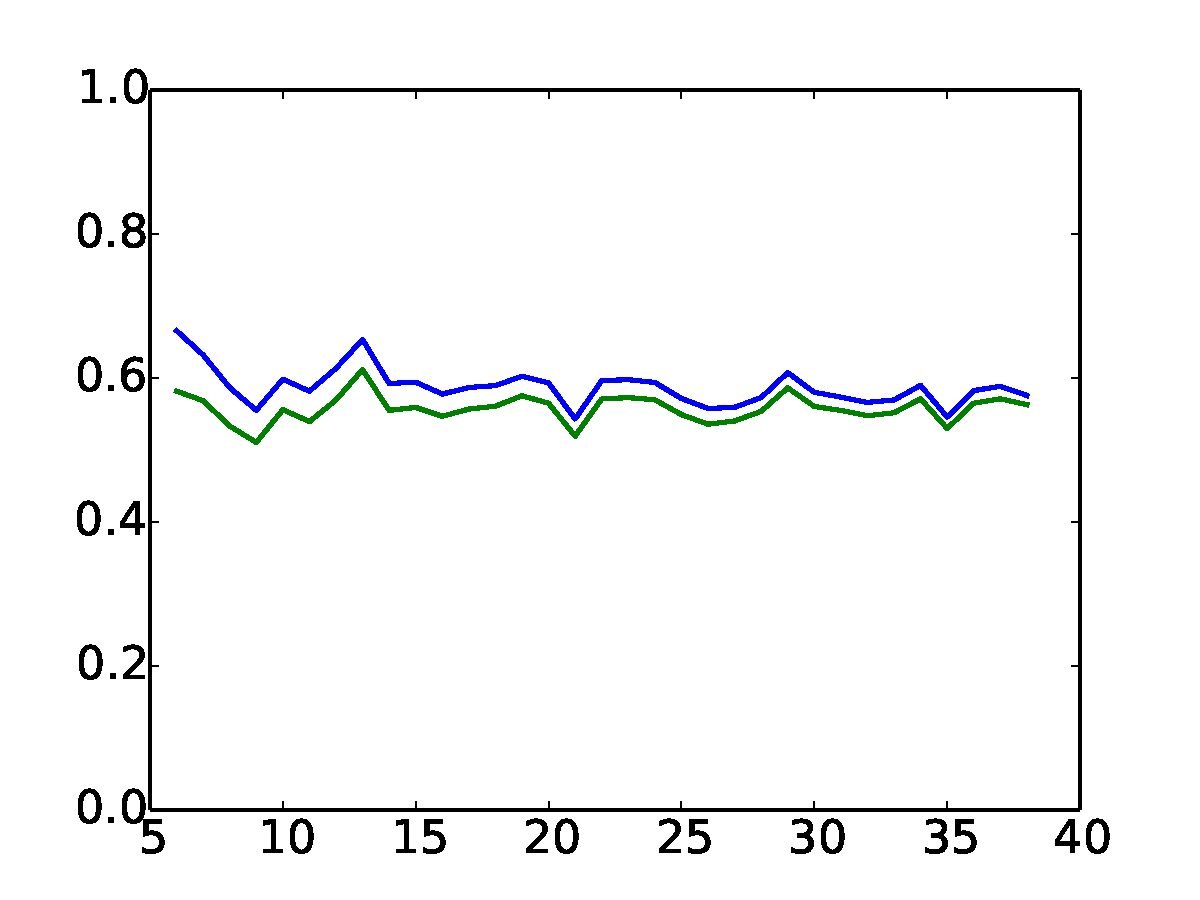
\includegraphics[width=0.8\textwidth]{true_value_test_standard}
		\caption{Верхняя и нижняя оценки стоимости опциона по алгоритму Броади-Глассермана}
		\label{fig:true_value_test_standard}
		\footnotesize{Оценки стоимости опциона с начальной ценой 100, выписанного на срок 1 год на базовый актив с риск-нейтральной процентной ставкой $r = 0.05$, дивидендной ставкой $\delta = 0.1$ и волатильностью $\sigma=0.2$, цена которого --- случайный процесс, являющийся геометрическим броуновским движением с параметрами $\mu = r - \delta$ и $\sigma$, исполняемого 4 раза в году}
	\end{figure}
	\par Наибольшая частота исполнения опциона, которую классическая оценка способна посчитать при разумных требованиях к памяти --- ежемесячно, $n=12$. Поэтому оценить этим алгоритмом стоимость американского опциона не представляется возможным.

\chapter{Устранение экспоненциальной сложности}
	\par Начиная с некоторого момента $t_k$, когда общее число состояний достигнет некоторого $n$, мы перестанем генерировать дочерние вершины ко всем состояниям. В следующий момент времени, $t_{k+1}$, мы будем иметь всё так же $n$ состояний, а не $bn$. Есть несколько способов сделать это, в том числе --- ограничивать множество состояний, в которые может перейти базовый актив.
	\section{Анализ распределения состояний с помощью эмпирической функции распределения}
	    \subsection{Описание метода}
        \par В том случае, когда состояние актива $S$ является числом в $\R ^1$, в качестве параметра $X$, по распределению которого мы составляем эмпирическую функцию распределения, можно использовать  само $S$, иначе можно использовать $h(S)$.
        \par Пусть мы промоделировали дерево состояний базового актива до момента $t_{k-1}$. Тогда определено множество состояний актива в момент времени $t_{k-1}$: $\left\lbrace S_j \right\rbrace_{j=1}^n, n=b^{i-1}$. Промоделировав у каждой $j\in 1:n$ вершины $b$ дочерних вершин (независимых реализаций процесса изменения состояния актива) $\left\lbrace S_j^i\right\rbrace_{i=1}^b$, получим множество $\left\lbrace\left\lbrace S_j^i \right\rbrace_{i=1}^b\right\rbrace_{j=1}^n$. Эмпирическая функция распределения состояния базового актива выглядит как
        $$F_{S}(x) = \frac{1}{bk}\#\left\lbrace (i, j) \in 1:b \times 1:k \middle\vert S_i^j < x \right\rbrace.$$
        Тогда мы можем сгруппировать вершины по квантилям их эмпирического распределения:
        $$\forall k\in 1:n \;\; A_k = \left\lbrace S_i^j \middle\vert \frac{k-1}{n} \leq F_{S}(S_i^j) < \frac{k}{n}\right\rbrace.$$
        У каждой группы однозначно определена медиана: либо среднее наблюдение в группе, либо смесь двух наиболее близких к середне. Заменяя всех членов группы её медианой, мы получаем $bn$ вершин вместо $n$. Процесс проиллюстрирован на рис. \ref{fig:reduceTree}.
        \begin{figure}[h]
		\begin{tikzpicture}[->,>=stealth',shorten >=1pt,auto,node distance=0.35\linewidth, main node/.style={rectangle,draw}]

            \node[main node] (2) {97}
                child { node[main node] (88) {88}}
                child { node[main node] (92) {92}}
                child { node[main node] (106) {106}};
            \node[main node] (3) [right of=2] {103}
                child { node[main node] (96) {96}}
                child { node[main node] (115) {115}}
                child { node[main node] (107) {107}};
            \node[main node] (1) [right of=3] {110}
                child { node[main node] (116) {116}}
                child { node[main node] (104) {104}}
                child { node[main node] (112) {112}};

            \node[main node] (92s) [below=0.1\paperheight of 92]{92}
                child { node[main node] (92r) {92}};
            \path (92) edge[<->] (92s);
            \node[main node] (88s) [below=0.1\paperheight of 88] {88};
            \path (88) edge[<->] (88s)
                (88s) edge (92r);
            \node[main node] (96s) [below=0.1\paperheight of 106]{96};
            \path (96) edge[<->] (96s)
                (96s) edge (92r);

            \node[main node] (106s) [below=0.1\paperheight of 115]{106}
                child { node[main node] (106r) {106}};
            \path (106) edge[<->] (106s);
            \node[main node] (104s) [below=0.1\paperheight of 96]{104};
            \path (104) edge[<->] (104s)
                (104s) edge (106r);
            \node[main node] (107s) [below=0.1\paperheight of 107]{107};
            \path (107) edge[<->] (107s)
                (107s) edge (106r);

            \node[main node] (115s) [below=0.1\paperheight of 104]{115}
                child { node[main node] (115r) {115}};
            \path (115) edge[<->] (115s);
            \node[main node] (112s) [below=0.1\paperheight of 116]{112};
            \path (112) edge[<->] (112s)
                (112s) edge (115r);
            \node[main node] (116s) [below=0.1\paperheight of 112]{116};
            \path (116) edge[<->] (116s)
                (116s) edge (115r);

        \end{tikzpicture}
		\caption{Выбор вершин по квантилям эмпирического распределения}
		\label{fig:reduceTree}
	    \end{figure}
		\par Таким образом, количество рассматриваемых состояний не увеличится. С другой стороны, этот метод предполагает хранение в памяти всего дерева, а не только непосредственно обсчитываемой ветки, как это предполагалось в исходной работе \cite{Broadie1997}.
		\par Также стоит отметить, что, пользуясь таким (и подобными ему) методом выбора состояний процесса, мы существенно нарушаем предположение об условной независимости реализаций: теперь состояние актива в $t_i$ зависит не только от состояния актива в $t_{i-1}$, но и от состояния этого актива в других реализациях процесса. Доказательство сходимости оценок $\hat{V}_0(S_0)$ и $\hat{v}_0(S_0)$ к $V_0(S_0)$ строится на том, что $\hat{V}_{i+1}^{j_1\cdots j_i 1}, \ldots \hat{V}_{i+1}^{j_1\cdots j_i b}$ при данном $S_i^{j_1\cdots j_1}$ --- независимые одинаково распределённые случайные величины с математическим ожиданием $\ev\left[V_{i+1}\left(S_{i+1}\right)\middle\vert S_i^{j_1\cdots j_1}\right]$. Следовательно, всё, чего мы можем ожидать, не меняя структуру оценок --- достаточно слабой корреляции.
		\par Генерирование каждого следующего ряда занимает $O\left(bn\log\left(bn\right)\right)$ времени (самая времязатратная операция --- сортировка массива сгенерированных вершин длины $bn$) и $O\left(bn\right)$ памяти, следовательно, сложность моделирования в целом составляет $O\left(mbn\log\left(bn\right)\right)$
		\subsection{Численные результаты}
		Алгоритм также реализован, принципиальная часть представлена в приложении \ref{lst:treeGeneration}. Результаты моделирования для оценки стоимости того же опциона, что был использован для демонстрации классического алгоритма, представлены на рис. \ref{fig:true_value_test_empiric_distr}
		\begin{figure}[h]
    	    \centering
    		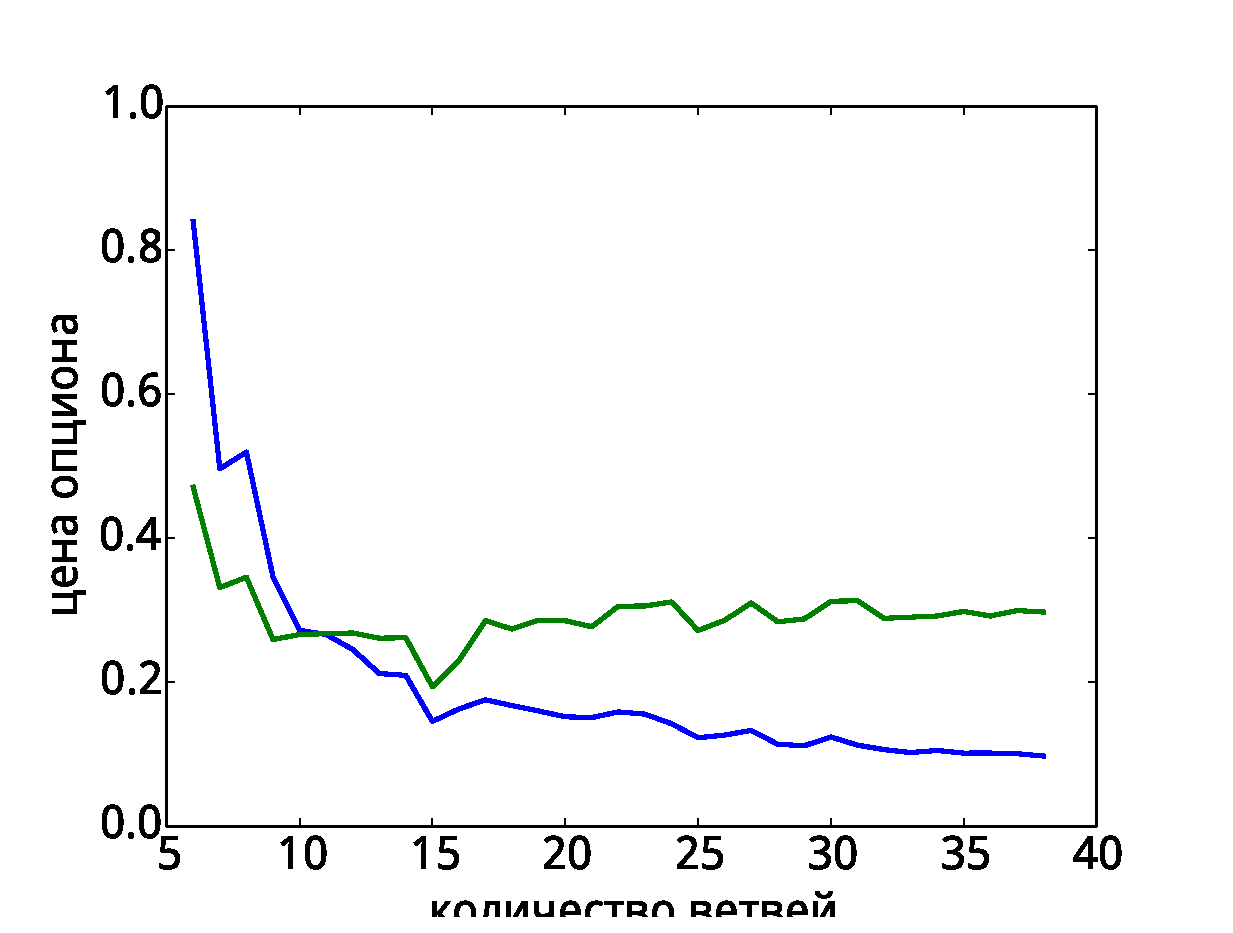
\includegraphics[width=0.8\textwidth]{true_value_test_empiric_distr}
    		\caption{Верхняя и нижняя оценки стоимости опциона по дереву с анализом эмпирической функцией распределения}
    		\label{fig:true_value_test_empiric_distr}
    		\footnotesize{Оценки стоимости опциона с начальной ценой 100, выписанного на срок 1 год на базовый актив с риск-нейтральной процентной ставкой $r = 0.05$, дивидендной ставкой $\delta = 0.1$ и волатильностью $\sigma=0.2$, цена которого --- случайный процесс, являющийся геометрическим броуновским движением с параметрами $\mu = r - \delta$ и $\sigma$, исполняемого 4 раза в году}
	    \end{figure}
		Из графика видно, что сходимости к истинному значению не наблюдается.
	\section{Конечная сетка состояний}
	    \subsection{Описание метода}
	        Для того, чтобы сложность алгоритма по  памяти составляла $O(bm)$, необходимо начиная с некоторого момента ограничивать множество состояний, в которые может перейти актив из данного. Так как мы имеем дело с нестационарным случайным процессом, распределение состояний на следующем шаге меняется, как только мы получаем новую реализацию состояния на предыдущем шаге.

	        Можно использовать знания о законе распределения, которому подчиняется состояние базового актива, чтобы уменьшить число возможных состояний.
	        $$dS_t = \mu S_t dt + \sigma S_t dW_t \implies \log \left(\frac{S_t}{S_0}\right)\sim N\left(\left(\mu - \frac{\sigma^2}{2}\right)t, \sigma^2 t\right).$$
	        Ограничив множество состояний базового актива в момент времени $t$ числом $n$, мы можем рассчитать, попадание в какие $n$ классов состояний будет равновероятно. Пусть $F(x)$ --- функция распределения $N\left(0, 1\right)$, тогда
	        \begin{align}
	            \forall i \in 1:n \;\;\exists\; \xi_i = F^{-1}\left(\frac{i-0.5}{n}\right) \text{ --- представитель $i$-го состояния} ,\\
	            \forall i \in 0:n \;\;\exists\; z_i = F^{-1}\left(\frac{i}{n}\right) \text{ --- граница $i$-го состояния} .
	        \end{align}
	        Для каждого момента времени $t_i$ определено множество состояний $$S_i^j = S_0\exp\left(\left(\mu - \frac{\sigma^2}{2}\right)t + \sigma \sqrt{t}\xi_j\right), j\in 1:n$$ и множество границ этих состояний $$Z_i^j = S_0\exp\left(\left(\mu - \frac{\sigma^2}{2}\right)t + \sigma \sqrt{t}z_j\right), j\in 1:n.$$
	        Для любого состояния $S_i^{j_1\cdots j_i}$ найдётся $k\in 1:n : Z_i^{k-1} \leq S_i^{j_1\cdots j_i} < Z_i^k$, тогда $S_i^{j_1\cdots j_i} := S_i^j$. Иллюстрация процесса --- на рис.\ref{fig:grid}
	        \begin{figure}[h]
        	    \centering
        		\caption{Дискретизация по квантилям $GBM(\mu, \sigma)$}
        		\label{fig:grid}
        	\end{figure}
	        Множество состояний не зависит от имеющихся результатов моделирования, только от параметров базового актива, следовательно, генерируемые траектории будут достаточно независимы, чтобы подходить под условия сходимости оценок \eqref{eq:upper}, \eqref{eq:lower}. Количество возможных состояний на каждом шаге можно увеличивать по мере увеличения $t_i$, что может частично компенсировать растущую дисперсию.
	        \subsection{Численные результаты}
	            Результаты моделирования для оценки стоимости того же опциона, что был использован для демонстрации классического алгоритма, представлены на рис. \ref{fig:true_value_test_finite_grid}
                \begin{figure}[h]
                    \centering
                    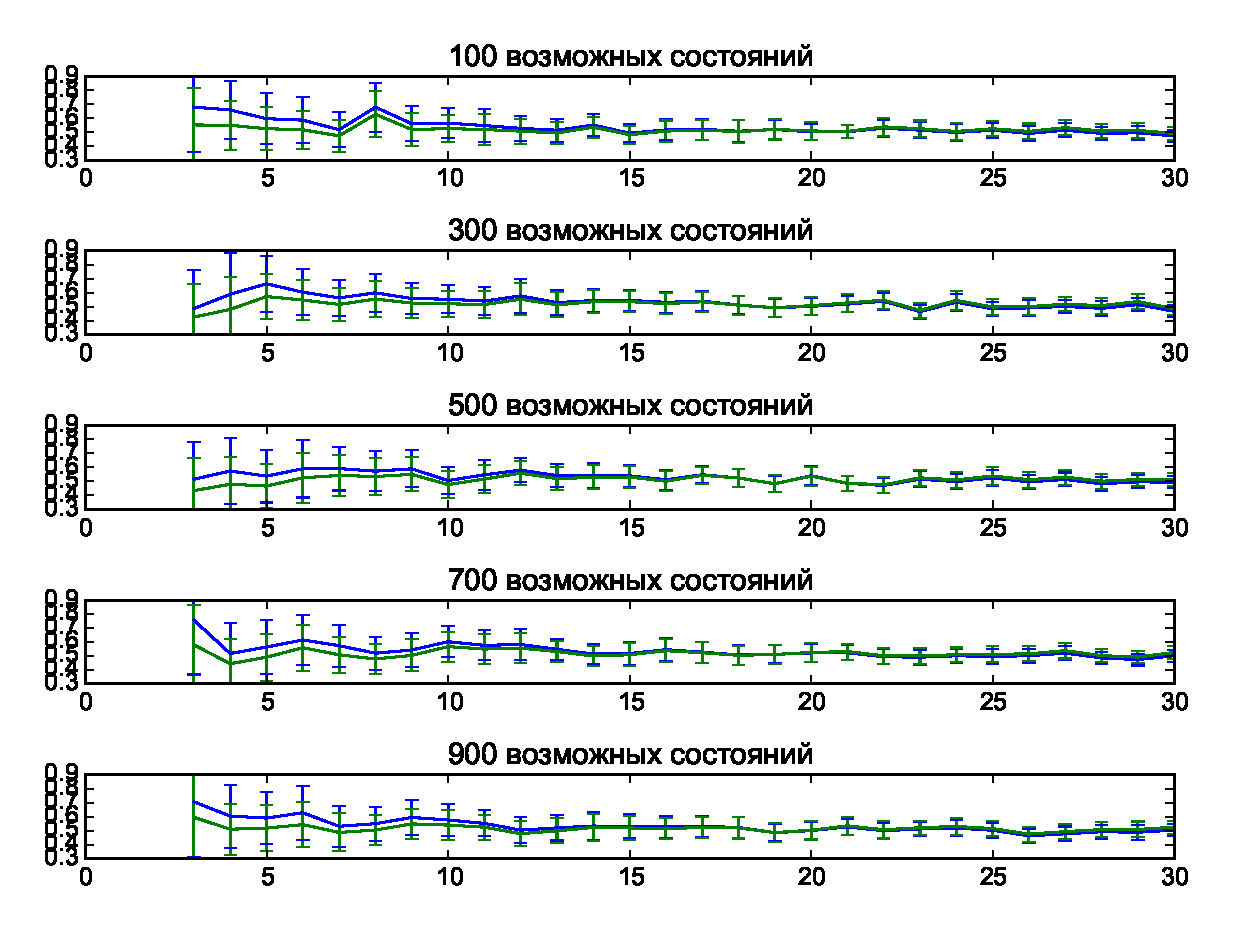
\includegraphics[width=\textwidth]{true_value_test_finite_grid}
                    \caption{Верхняя и нижняя оценки стоимости опциона по дереву с анализом эмпирической функцией распределения}
                    \label{fig:true_value_test_finite_grid}
                    \footnotesize{Оценки стоимости опциона с начальной ценой 100, выписанного на срок 1 год на базовый актив с риск-нейтральной процентной ставкой $r = 0.05$, дивидендной ставкой $\delta = 0.1$ и волатильностью $\sigma=0.2$, цена которого --- случайный процесс, являющийся геометрическим броуновским движением с параметрами $\mu = r - \delta$ и $\sigma$, исполняемого 4 раза в году}
                \end{figure}
                Несмотря на выполнение условий сходимости, налагаемых на траектории, вычисления демонстрируют отсутствие сходимости при $b \to \infty$: при больших значениях $b$ ($b=60, 80$, не показаны на графике) оценки демонстрируют устойчивое поведение, и среднее значение верхней и нижней оценки по 100 реализаций для каждого $b$ равны $0.48\pm 0.02$ и $0.43\pm 0.03$ соответственно.




\section*{Дальнейшие планы}
	\begin{enumerate}
		\item Посчитать конечную сетку
		\item Рассмотреть метод взвешивания траекторий (количество дочерних вершин, которое позволено иметь вершины, пропорционально её вкладу в общую оценку)
	\end{enumerate}
\nocite{*}
\bibliographystyle{ugost2008}
\bibliography{biblio-u}

\appendix
\chapter{Реализация на Java}
Моделирование организовано итеративно (а не рекурсивно, как это было бы уместно в исходном методе), потому что необходимая информация о дереве в процессе моделирования --- это описание текущего ряда целиком. Поэтому проще всего --- пройти вниз по дереву один раз.
% % \renewcommand{\lstlistingname}{Листинг}% Listing -> Algorithm
% \renewcommand{\lstlistlistingname}{Листинги}
\begin{lstlisting}[caption={Генерирование дерева состояний актива, на который выписан опцион},label={lst:treeGeneration}]
public static ImitatedAsset generateAssetTree(int branches, int steps, double initialPrice){
        timedelta = 1. / steps;
        ImitatedAsset ans = new ImitatedAsset(initialPrice, branches, false, timedelta);
        ImitatedAsset[] prevRow = getFirstRow(ans, branches);
        for (int step = 0; step < steps; step++) {
            boolean median = branches % 2 == 1;
            ImitatedAsset[] curRow = new ImitatedAsset[branches * prevRow.length];
            ImitatedAsset[] newRow = new ImitatedAsset[prevRow.length];
            for (int i = 0; i < prevRow.length; i++) {
                for (int b = 0; b < branches; b++) {
                    curRow[i * branches + b] = new ImitatedAsset(getRandomPrice(prevRow[i]), branches, false, timedelta);
                    curRow[i * branches + b].parent = prevRow[i];}}
            Arrays.sort(curRow);
            for (int i = 0; i < prevRow.length; i++) {
                ImitatedAsset v;
                if (median) {
                    v = curRow[i * branches + branches / 2 + 1];
                } else {
                    double price = (
                            curRow[i * branches + branches / 2].price + curRow[i * branches + branches / 2 + 1].price
                    ) / 2;
                    v = new ImitatedAsset(price, branches, false, timedelta);}
                for (int b = 0; b < branches; b++) {
                    curRow[i * branches + b].parent.addChild(v);
                    curRow[i * branches + b] = null;}
                newRow[i] = v;}
            prevRow = newRow;}
        return ans;}
\end{lstlisting}

\end{document}
